\subsection{Erste Implementation}

Die jetzige Methode, ein Polygonnetz der Voxels
zu erstellen besteht darin, für jeden Voxel
ein Würfelnetz zu erstellen.
Um dies also zu cullen, überprüft man
noch die Nachbarvoxels, um zu entscheiden,
welche Seiten sichtbar sind, und erstellt nur
die sichtbaren Seiten.

\begin{figure}[ht]
	\begin{minipage}[c]{0.49\textwidth}
		\begin{center}
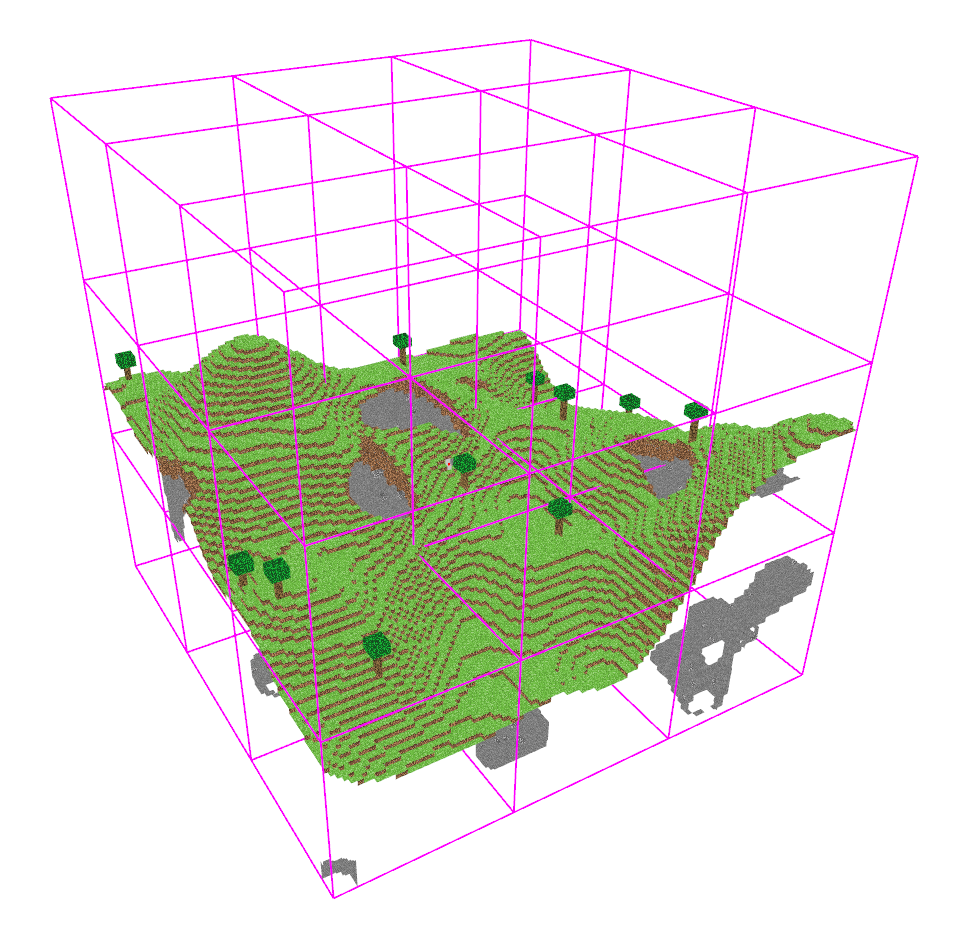
\includegraphics[width=0.8\textwidth]{../assets/culling/chunk_borders.png}
		\end{center}
	\end{minipage}
	\begin{minipage}[c]{0.49\textwidth}
Da die Spielwelt unendlich groß ist, muss sie
in viele einzelne Polygonnetze aufgeteilt werden.
Somit ist die Welt in sogenannte \gqq{Chunks}
eingeteilt, die $32 \times 32 \times 32$ Voxels
beinhalten. Das Polygonnetz, das die Voxels in einem
Chunk anzeigt, werde ich als
\gqq{Chunknetz} bezeichnen.
	\end{minipage}\hfill
\end{figure}

Da das Erstellen eines Chunknetzes lang dauern kann,
soll das Spiel nicht darauf warten,
da dies sonst sichtbar beim Spielen wäre.
Deswegen werden die Chunknetze in separaten
\href{https://de.wikipedia.org/wiki/Thread_(Informatik)}{Threads}
\cite{wiki_thread} erstellt.
Zudem können somit mehrere Chunknetze gleichzeitig
erstellt werden.

Wir brauchen also erst Zeit, um den Thread zu starten,
und dann verwenden wir die meiste Zeit, um das
Chunknetz zu erstellen.
Wir erhalten folgende Performance:

\vspace{0.3cm}

% dont know how to get rid of this
% warning or what it means
% Erste Implementation stats from: bench 01
\benchgraph{1}{0.0}{
	algo                   & blue       & red       \\
	Erste Implementation   & 12.834184  & 0.672563  \\
}

\vspace{0.3cm}

Dadurch entsteht aber ein neues Problem: \\
Wenn mehrere Threads zugriff auf die gleichen Daten
haben, muss dieser Zugriff synchronisiert werden,
da sonst eine
\href{https://de.wikipedia.org/wiki/Wettlaufsituation}{Wettlaufsituation}
\cite{wiki_wettlauf} (genauer gesagt ein Data Race)
entstehen kann \cite{nomicon_races}.
Durch diese Synchronisierung müsste aber jeder Zugriff
zu Chunks auf andere Threads warten, was das gesamte
Spiel langsamer machen würde. Deswegen werden die
Daten der nötigen Chunks zu dem Thread kopiert,
was langsam ist, da es sich hier um sehr große Daten
handelt.

Culling braucht Information aus den benachbarten
Chunks, um zu entscheiden, ob die Ränder des Chunks
sichtbar sind. Somit müssen die 6 Nachbarchunks
auch zu dem Thread kopiert werden, was sehr viele
Daten sind. Man könnte zwar nur die Voxels
kopieren, die am Rand des Chunks sind,
aber wir werden gleich eine Methode sehen,
die dieses Problem und andere auf einmal löst.

\vspace{0.3cm}

Ein weiteres Problem besteht darin, dass dieser
Algorithmus für jeden Voxel noch die 6 Nachbarn
betrachten muss. Somit wird jeder Voxel 7-mal
betrachtet.
